\documentclass[a4paper,slidestop,xcolor=pst,blue]{beamer}

\usepackage{beamerthemesplit}
\usepackage[utf8]{inputenc}
\usepackage[spanish]{babel}
\usepackage{graphicx}
\usepackage{pstricks} % PSTricks package
\usepackage{setspace}
\usepackage{multirow}
\usepackage{listings}
\usepackage{pgfpages}
\usepackage{hyperref}
\usepackage{etoolbox}
\usepackage{epstopdf}

\makeatletter
\patchcmd{\beamer@sectionintoc}{\vskip1.5em}{\vskip0.5em}{}{}
\makeatother

\setbeamercovered{dynamic}
\setcounter{tocdepth}{2}
\setbeamercolor{frametitle}{fg=black,bg=white}
\setbeamercolor{section in toc shaded}{fg=black}
\setbeamercolor{section in toc}{fg=red}
\setbeamercolor{subsection in toc shaded}{fg=black}
\setbeamercolor{subsection in toc}{fg=red}
\setbeamerfont{section in toc}{size=\small}
\setbeamerfont{subsection in toc}{size=\small}
\setbeamertemplate{section in toc shaded}[default][99]
\setbeamertemplate{subsection in toc shaded}[default][99]

\AtBeginSection[]
{\begin{frame}[c]
  \frametitle{Índice}
	\tableofcontents[currentsection,
        sectionstyle=show/shaded,
        subsectionstyle=hide]
\end{frame}}

\AtBeginSubsection[]
{\begin{frame}[c]
	\frametitle{Índice}
	\tableofcontents[
  		currentsection,
  		sectionstyle=shaded/shaded,
  		currentsubsection,
  		subsectionstyle=show/shaded/hide
		]
\end{frame}}

\setbeamercolor{frametitle}{fg=black,bg=white}

\setbeamertemplate{frametitle}{
	\begin{centering}
		\insertframetitle
		\par
	\end{centering}
}

\usetheme[secheader]{Boadilla} 

\title[Capa de Servicio - Fundamentos]{Capa de Servicio - Fundamentos }

\author[P. S{\'a}nchez]{\alert{Pablo S{\'a}nchez}}

\institute[IIE]{
		   Dpto. Ingenier{\'i}a Inform{\'a}tica y Electr{\'o}nica \\
		   Universidad de Cantabria \\
		   Santander (Cantabria, Espa{\~n}a) \\
		   \texttt{p.sanchez@unican.es}
}

\date{}

\begin{document}

\begin{frame}[c]
	\titlepage
	\begin{columns}
		\column{0.50\linewidth}
			\centering
    		
\includegraphics[width=.28\textwidth,keepaspectratio=true]{images/istr.eps}
		\column{0.50\linewidth}
			\centering
			
\includegraphics[width=.25\textwidth,keepaspectratio=true]{images/uc.eps}
	\end{columns}
\end{frame}

\begin{frame}[c]
    \frametitle{\alert{Advertencia}}
    \begin{center}
        Todo el material contenido en este documento no constituye en modo alguno una obra de referencia o apuntes oficiales mediante el cual se puedan preparar las pruebas evaluables necesarias para superar la asignatura. \ \\
        \ \\
        Este documento contiene exclusivamente una serie de diapositivas cuyo objetivo es servir de complemento visual a las actividades realizadas en el aula para la transmisi{\'o}n del contenido sobre el cual versar{\'a}n las mencionadas pruebas evaluables.  \ \\
        \ \\
        Dicho de forma m{\'a}s clara, \alert{estas transparencias no son apuntes y su objetivo no es servir para que el alumno pueda preparar la asignatura.}
    \end{center}
\end{frame}

\section{Introducción}

\begin{frame}
    \frametitle{Capa de Servicio}
    \only<1|handout:2>{
        \rput[lt](0,0){
            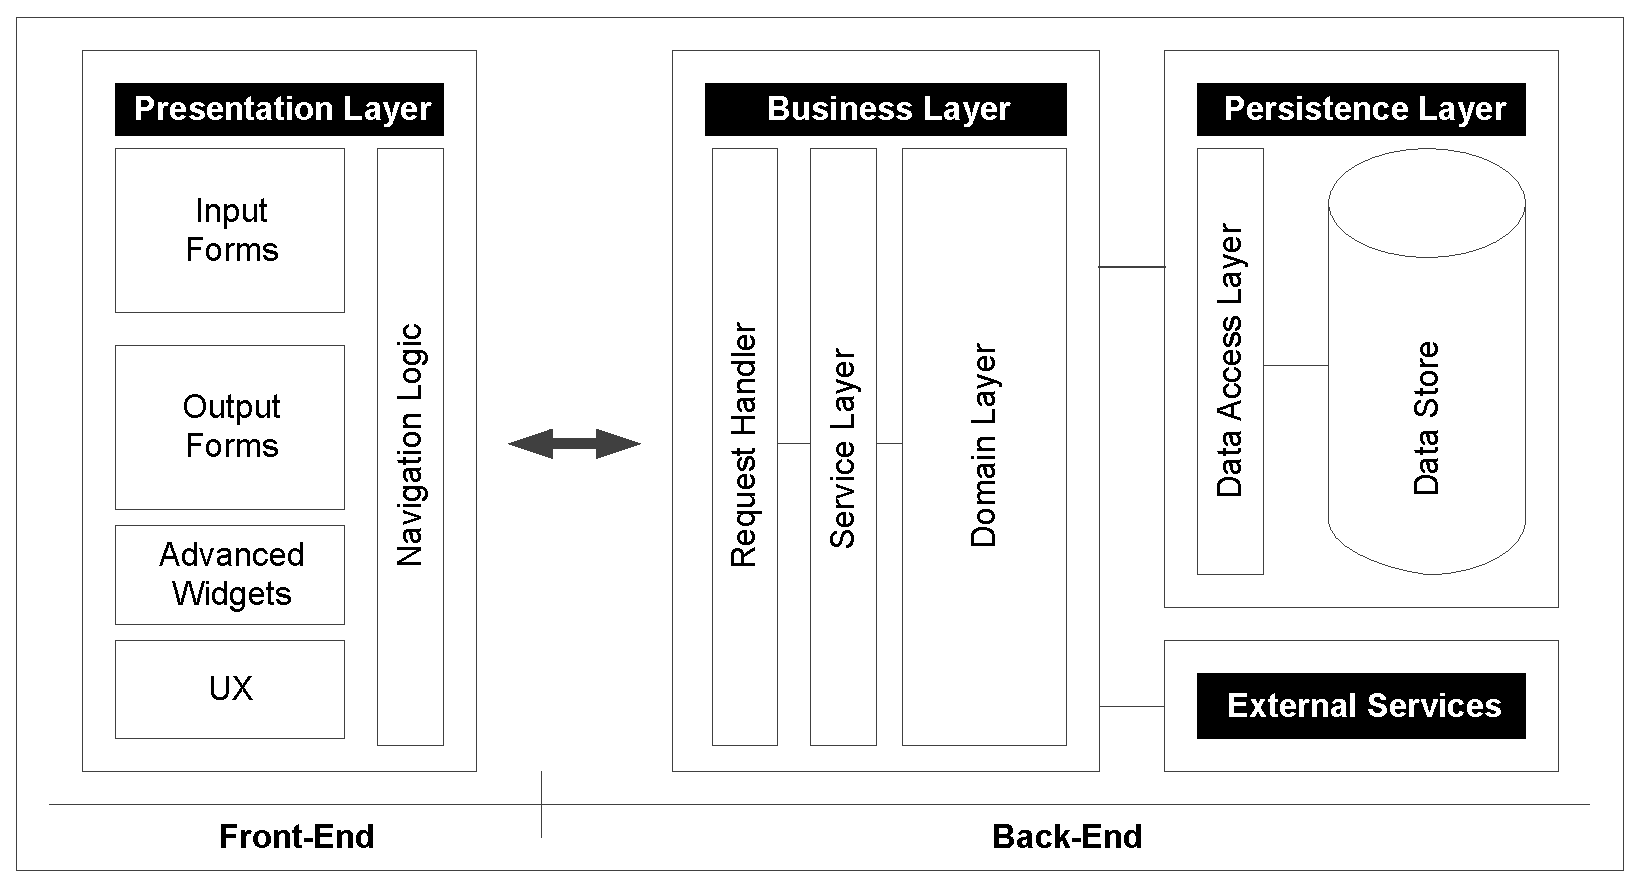
\includegraphics[width=\linewidth]{images/intro/enterpriseArchitectures00.eps}
        }
    }
    \only<2|handout:2>{
        \rput[lt](0,0){
            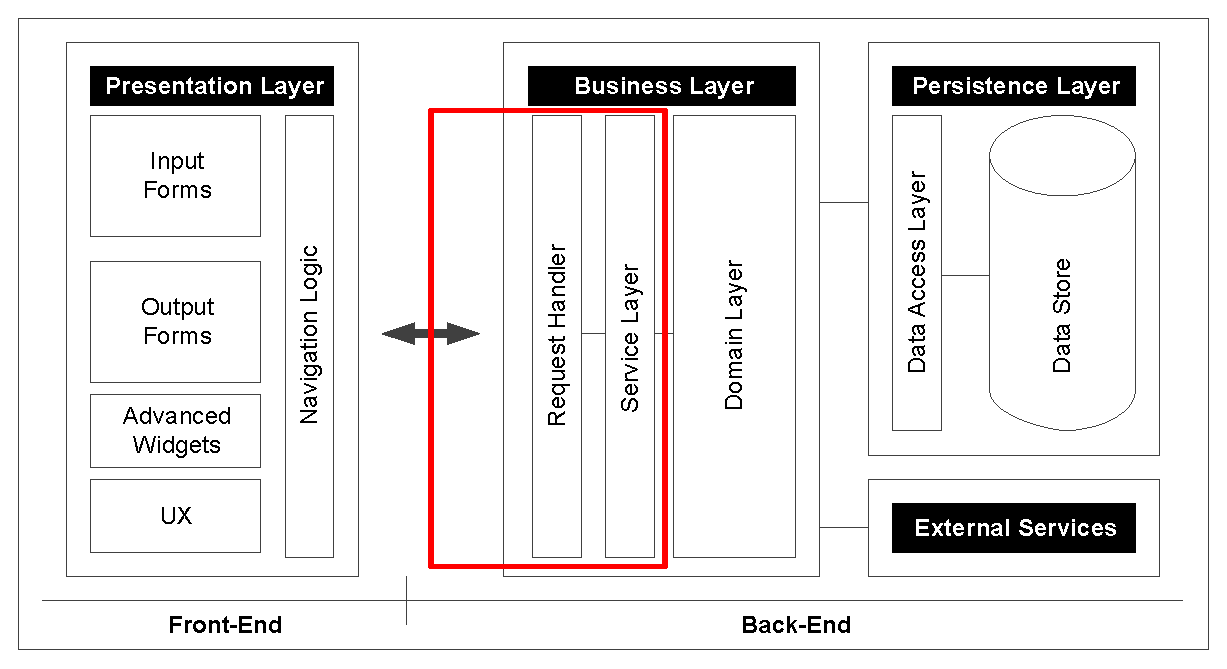
\includegraphics[width=\linewidth]{images/intro/enterpriseArchitectures01.eps}
        }
    }
\end{frame}

\begin{frame}[c]
	\frametitle{Responsabilidades de la Capa de Servicio}
	\begin{enumerate}[<+->]
        \item Atender las peticiones HTTP de los clientes, delegando en el modelo de dominio.
        \item Asegurar la transaccionalidad de las operaciones de negocio.
        \item Validar las peticiones de los clientes.
        \item Recuperar y almacenar datos del almacén o almacenes persistentes.
        \item Facilitar la eficiencia del sistema.
        \item Controlar el acceso a los datos.
        \item Gestionar la comunicación con los servicios externos.
        \item Gestionar de manera adecuada casos excepcionales.
        \item Ayudar a satisfacer los requisitos no funcionales.
	\end{enumerate}
\end{frame}

\begin{frame}[c]
    \frametitle{Objetivos del Tema}
    \begin{enumerate}[<+->]
         \item Comprender en profundidad cuáles son las responsabilidades de la capa de servicio.
         \item Comprender cómo funciona el protocolo HTTP.
         \item Comprender los principios de las arquitecturas REST.
         \item Saber diseñar una API REST.
         \item Ser capaz de usar los patrones de diseño propios del diseño de una capa de servicio.
    \end{enumerate}
\end{frame}

\begin{frame}[c]
    \frametitle{Bibliografía}
    \begin{thebibliography}{1}

        \bibitem[Fowler, 2002]{Fowler2002}
        Fowler, M. (2002).
        \newblock {\em {Patterns of Enterprise Application Architecture}}.
        \newblock Addison-Wesley.

        \bibitem[Esposito and Saltarello, 2014]{Esposito2014}
        Esposito, D. y Saltarello, A. (2014).
        \newblock {\em {Microsoft .NET - Architecting Applications for the
          Enterprise}}. 2ª Ed..
        \newblock Microsoft Press

        \bibitem{Ricahrdson2007}
        Richardson, L. and Ruby, S.
        \newblock {\em {RESTful Web Services}}.
        \newblock  O'Reilly, 2007.

    \end{thebibliography}
\end{frame}

\section{Arquitecturas y Controladores REST}

\subsection{Introducción}

\begin{frame}
    \frametitle{Controlador HTTP}
    \only<2|handout:2>{
        \rput[lt](0,0){
            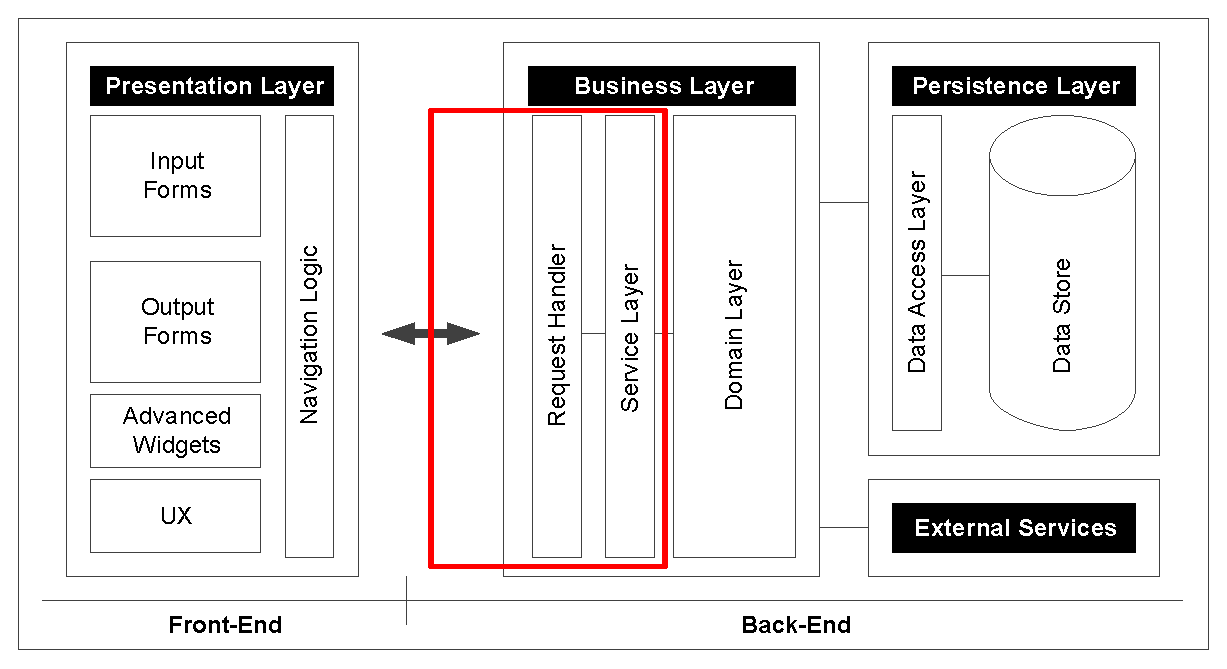
\includegraphics[width=\linewidth]{images/intro/enterpriseArchitectures01.eps}
        }
    }
\end{frame}

\begin{frame}[c]
	\frametitle{Responsabilidades del Controlador HTTP}
	\begin{enumerate}[<+->]
        \item Atender las peticiones HTTP de los clientes.
        \item Convertir datos de HTTP al lenguaje que corresponda (\emph{unmarshalling}).
        \item Validar las peticiones de los clientes.
        \item Convertir las respuestas a una respuesta HTTP adecuada.
        \item Convertir los resultados a datos HTTP (\emph{marshalling}).
	\end{enumerate}
\end{frame}

\subsection{Arquitectura REST}

\begin{frame}[c]
	\frametitle{Arquitectura REST}
	\begin{block}{Sistema Hipermedia}
        Un \emph{sistema hipermedia} fusiona información de control de la aplicación con la presentación de la información.
	\end{block}
    \uncover<2->{
    	\begin{block}{REST \emph{(REpresentational State Transfer)}
            \begin{enumerate}[<+->]
                \item  REST es un estilo arquitectónico diseñado para satisfacer las necesidades de los sistemas de hipermedia a escala de internet.
                \item Una \emph{aplicación web} se concibe como una máquina de estados donde el usuario progresa mediante la selección de links y el envío de formularios.
                \item La representación de cada estado se transfiere al usuario.
    	\end{block}
    }
\end{frame}

\begin{frame}[c]
	\frametitle{Objetivos Arquitectura REST}
    \begin{enumerate}
        %% Enlaces
        \item Minimizar latencias.
        %% Escalabilidad
        \item Trata de minimizar comunicaciones a nivel de red
        %% Altas cargas de usarios
        \item Maximiza la escalabilidad de los componentes
        %%
        \item Mazimiza la independencia de los componentes

        \item Permite cachear resultados e interacciones.
        \item Permite la sustitución dinámica de componentes
        \item Procesamiento de acciones por intermediarios
    \end{enumerate}
\end{frame}

\begin{frame}[c]
	\frametitle{Estilos Arquitectura REST}
    \begin{enumerate}[<+->]
        %% Presentación vs Almacenamiento y Procesamiento.
        %% Portabilidad
        %% Reemplazabilidad dinámica de comportamiento.
        \item Cliente-Servidor.
        %% El servidor no debe almacenar nada sobre el estado de los clientes.
        %% Cada petición del cliente debe tener toda la información necesaria para interpretarla.
        %% Favorece la escalabilidad.
        %% Favorece reliability (puedo volver a un estado anterior)
        %% Favore procesamiento por terceros.
        \item Stateless.
        %% Favorece el rendimiento
        \item Respuestas cacheables.
        %% Favorece la evolución
        %% Favorece la visibilidad
        \item Interfaces uniformes entre componentes.
        \item Código bajo demanda.
        \item Representación adaptable.
    \end{enumerate}
\end{frame}

\subsection{Recursos REST}

\begin{frame}[c]
	\frametitle{Recursos REST}
    \begin{block}{Recurso REST}
        Un \emph{recurso REST} es cualquier pieza de información a la que sea posible darle un nombre, que será el \emph{identificador del recurso}.
    \end{block}
    \uncover<2->{
        \begin{block}{Recurso REST}
            Una \emph{representación de recurso} es un conjunto de información que contiene datos, metadatos y, opcionalmente, metadatos sobre los metadatos.
        \end{block}
    }
\end{frame}

\begin{frame}[c]
	\frametitle{Representación de un Recurso REST}
    \begin{enumerate}
        \item Contiene datos de control (qué se debe hacer con el recurso).
        \item Contiene datos (asociados al control).
        \item Los datos pueden estar disponibles en varios formatos, abierto a negociación.
    \end{enumerate}
\end{frame}

%% Connector Stateless

%% (1) No necesita mantener estado.
%% (2) Facilita el procesamiento en paralelo.
%% (3) Permite interpretar la petición de manera aislada y realojar servicios.
%% (4) Permite la construcción de caches intermedias.

\section{Patrones de Servicio}

\subsection{Unit of Work}

\subsection{Data Transfer Object}

\section{Sumario}

\begin{frame}[c]
    \frametitle{¿Qué tengo que saber de todo ésto?}
    \begin{enumerate}[<+->]
        \item
    \end{enumerate}
\end{frame}

\end{document}
